\documentclass[10pt,twocolumn,letterpaper]{article}

\usepackage[margin=1.7cm,top=2.0cm,bottom=2.0cm,columnsep=0.65cm]{geometry}
\usepackage{times}
\usepackage{amsmath,amssymb,amsfonts}
\usepackage{graphicx}
\usepackage{booktabs}
\usepackage{microtype}
\usepackage{abstract}
\usepackage{xurl}
\usepackage{hyperref}
\usepackage{xcolor}
\usepackage{cite}
\usepackage{float}
\usepackage{titlesec}
\usepackage{tabularx}
\usepackage{balance}

% Figures produced by the notebook (saved next to it)
\graphicspath{{../notebooks/}{./notebooks/}{./}{../}{./figures/}}

\definecolor{navyblue}{RGB}{16, 44, 87}

\hypersetup{colorlinks=true, linkcolor=navyblue, citecolor=navyblue, urlcolor=navyblue}

\titleformat{\section}{\large\bfseries\color{navyblue}}{\thesection.}{0.5em}{}
\titleformat{\subsection}{\normalfont\bfseries\color{navyblue}}{\thesubsection}{0.5em}{}
\titlespacing*{\section}{0pt}{7pt}{2pt}
\titlespacing*{\subsection}{0pt}{4pt}{2pt}

\renewcommand{\abstracttextfont}{\normalfont\small\itshape}

\title{\huge \bfseries \color{navyblue} Predicting Workers' Compensation Claim Costs and Triaging Severe Claims at First Notice of Loss}

\author{
    \textbf{Marius Occhiminuti} \quad \textbf{Ga\"etan Amiens} \\
    School of Computer Science / Engineering, Reykjavik University \\
    \vspace{2pt} \\
    \small \textbf{Course Project:} Data Mining \& Machine Learning (DMML) \quad--\quad \textbf{Term:} Fall 2026
}
\date{}

\begin{document}
\maketitle

\begin{abstract}
At first notice of loss (FNOL), an insurer must estimate the ultimate cost of a workers' compensation claim and decide which
claims deserve a senior adjuster. Using 100,000 synthetic claims (OpenML 42876), we ask whether machine learning on the
information available at reporting time, including the free-text claim description, can do better than the adjuster's own
initial estimate. All model choices are made by 5-fold cross-validation (CV) on the training set with leak-proof pipelines;
the test set is used once. A tuned LightGBM on tabular features and TF-IDF text explains 45.8\% of the variance of the
log-cost on the test set (dollar-scale $R^2 = 0.024$, as expected for a target dominated by a few very large claims). For
triage of the 10\% most expensive claims, it reaches a ROC-AUC of 0.864 and a PR-AUC of 0.450, against 0.848 and 0.388 for
the adjuster's estimate, and flags claims carrying 46.4\% of total cost against 43.2\% at equal review capacity. The model
relies heavily on the initial estimate and inherits its errors: most missed severe claims had a low initial estimate. We
also show that back-transforming log predictions under-states portfolio totals by a factor of five, that a single Duan
smearing factor over-corrects because residuals are heteroscedastic, that costs drift with accident year, and that
removing sensitive attributes harms group calibration through proxy effects.
\end{abstract}

% =====================================================================
\section{Problem}
Workers' compensation insurance covers employees' medical costs and lost wages after a workplace injury. When a claim is
reported, the insurer sets an initial reserve and decides how to handle the file. Two questions follow:
\begin{enumerate}
    \item \textbf{Valuation (regression):} predict the ultimate incurred cost \texttt{UltimateIncurredClaimCost} from the
    information available at reporting time.
    \item \textbf{Triage (ranking):} identify the claims that will end in the top 10\% of costs, so that a limited number of
    senior adjusters can be assigned to them early.
\end{enumerate}

\paragraph{Framing fixed before modelling.} The unit is one claim at FNOL. Inputs are worker and employment attributes,
dates, the adjuster's \texttt{InitialCaseEstimate} (ICE) and the free-text \texttt{ClaimDescription}. Models are fitted on
$z=\log(1+y)$ because the cost is extremely right-skewed. A claim is \emph{severe} if its cost is at or above the 90th
percentile of the training costs (\$15,219). Metrics are MAE, RMSE and $R^2$ in dollars; RMSE and $R^2$ on the log scale;
and, for triage, ROC-AUC, PR-AUC (average precision) and \emph{loss capture@10\%}, the share of total cost contained in the
10\% of claims with the highest score. The \textbf{selection rule} is the lowest mean 5-fold CV RMSE on the log scale;
dollar RMSE is reported but not used to choose, because a handful of claims dominate it. Baselines are the mean and median
cost, the mean log-cost, and the adjuster, whose ICE is used both as a prediction and as a triage score.

% =====================================================================
\section{Data}
The dataset (OpenML 42876, \emph{workers\_compensation}~\cite{openml}) contains 100,000 claims and 14 raw variables.
It comes from the \emph{synthetic} workers' compensation data released for an actuarial data-science competition on
Kaggle~\cite{cas2020}. Currency, jurisdiction and inflation are not documented.

The cost is extremely concentrated: in the test set, the 2,016 severe claims (10.1\%) account for \$202.1M of the
\$227.9M total (88.7\%), and individual claims exceed \$1.6M. On the log scale the distribution is close to
symmetric (Figure~\ref{fig:target}), which motivates modelling $z=\log(1+y)$.

\begin{figure*}[t]
\centering
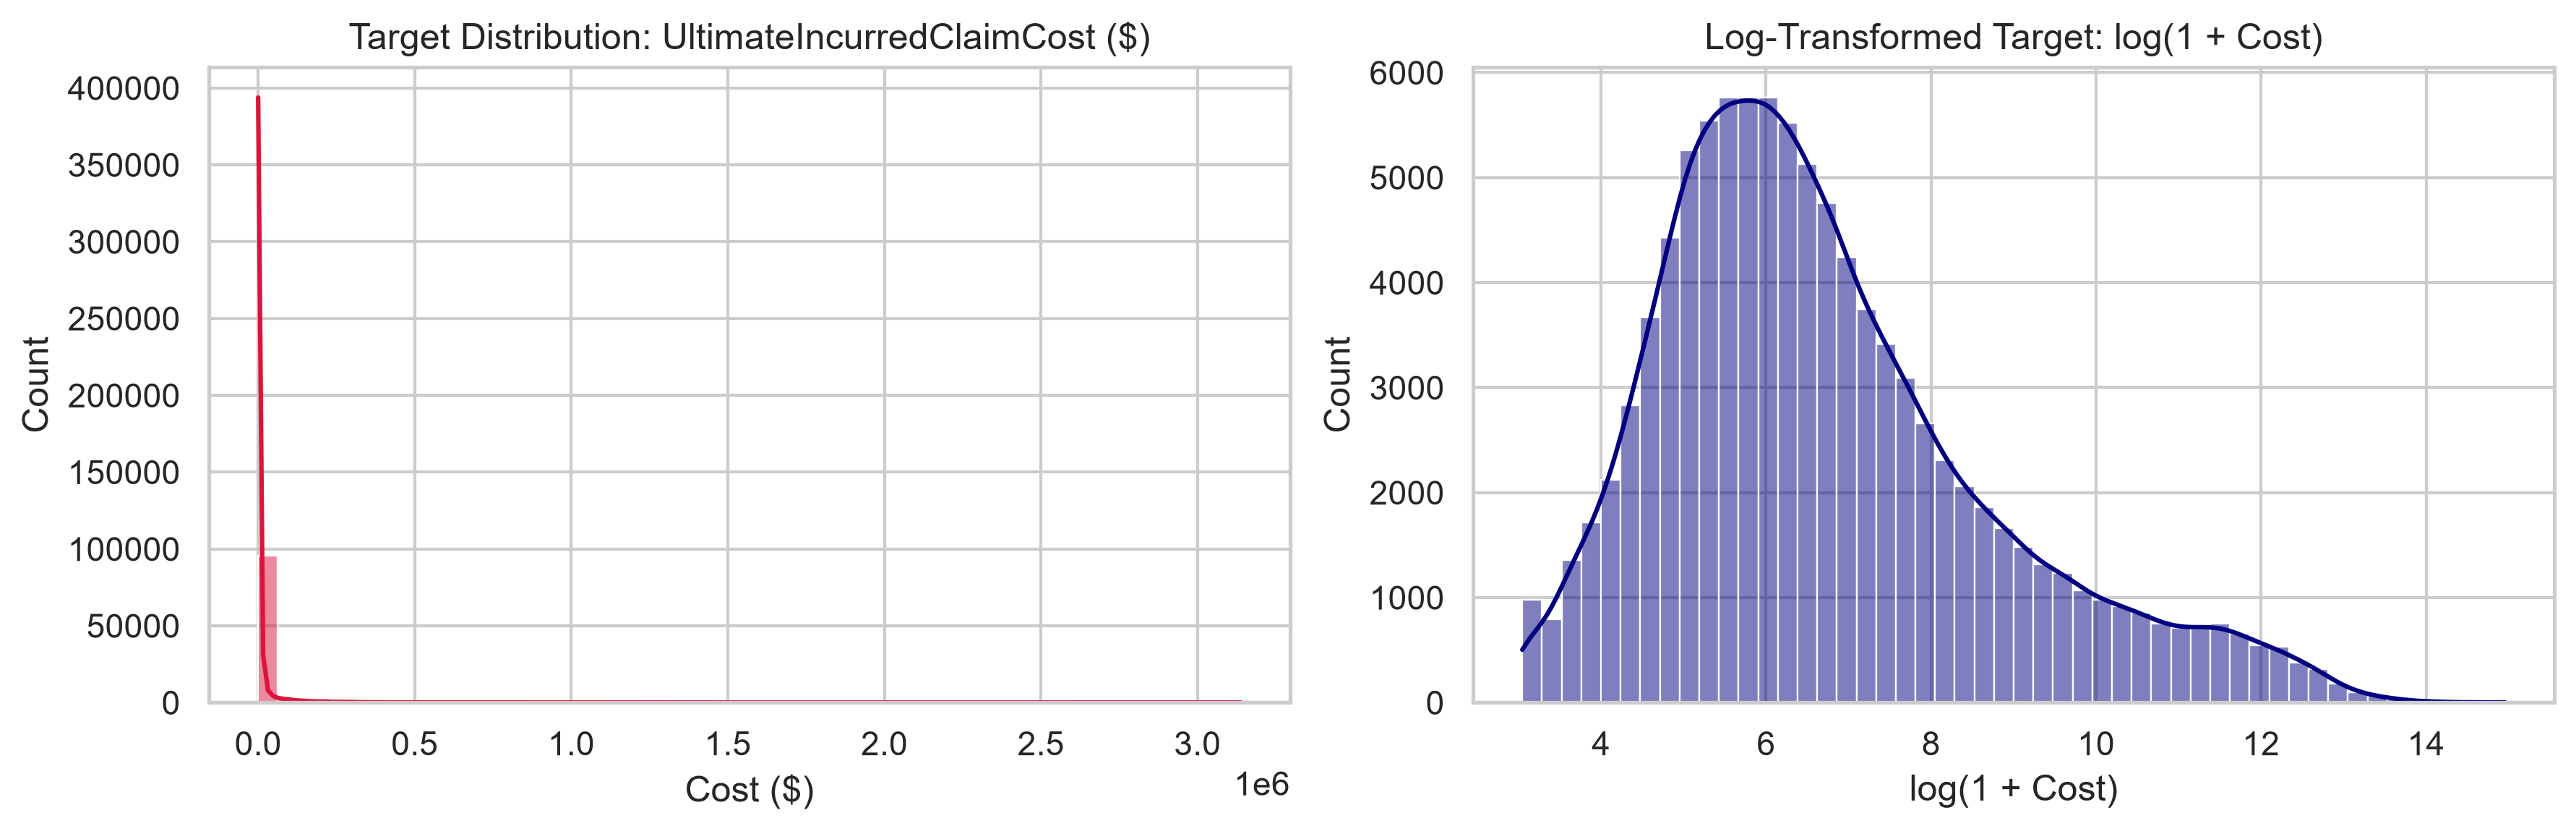
\includegraphics[width=0.82\linewidth]{fig_target_dist.png}
\caption{Distribution of the ultimate claim cost. Left: dollar scale. Right: $\log(1+\text{cost})$.}
\label{fig:target}
\end{figure*}

\paragraph{Features.} From the two dates we derive \texttt{ReportDelayDays} (reporting date minus accident time, floored at
zero) and the accident year, month, hour and weekday. Numeric inputs are \texttt{WeeklyPay}, \texttt{ReportDelayDays} and
ICE (all $\log(1+x)$ then robust-scaled), \texttt{Age}, hours and days worked per week, dependants, and the four date
features (robust-scaled). Categorical inputs (\texttt{Gender}, \texttt{MaritalStatus}, \texttt{PartTimeFullTime}) are
one-hot encoded. The description is represented by TF-IDF (unigrams and bigrams, 1,000 terms, $\text{min\_df}=5$), or by
its 50-component LSA (truncated SVD of the TF-IDF) for models that need dense inputs.

\paragraph{Split.} One random 80/20 split (seed 42): 80,000 training and 20,000 test claims. Five CV folds are drawn once
from the training set and reused by every model, so models can be compared fold by fold.

% =====================================================================
\section{Methods}
\paragraph{Leak-proof protocol.} Every transformation that learns from data (scalers, encoders, TF-IDF, SVD, feature
selection) sits inside a scikit-learn \texttt{Pipeline} and is refitted on the training part of each fold. All
comparisons, tuning and the choice of champion use the training folds only. The severity threshold is recomputed from
the training part of each fold. The test set is used once, after the champion is fixed.

\paragraph{Models.} Ridge regression (TF-IDF); random forest (tabular only); LightGBM with default settings on tabular
inputs and on tabular + TF-IDF; LightGBM tuned by randomised search (6 configurations, 3-fold CV, log-RMSE); the tuned
LightGBM~\cite{ke2017lightgbm} with an in-fold SHAP~\cite{lundberg2017shap} feature selector that keeps the 100 features with the largest mean $|\text{SHAP}|$ (the
ranking is recomputed inside every fold); a LightGBM with a Tweedie objective~\cite{jorgensen} (variance power 1.5) fitted directly on dollar
costs; and an MLP (two hidden layers of 128 and 64 units, early stopping) on tabular inputs and LSA text. A class-weighted
LightGBM classifier for the severe class is compared with ranking claims by the regression output. Model families do not
all see the same text representation, so differences between families mix model and input effects; the LightGBM rows
(tabular $\rightarrow$ +TF-IDF $\rightarrow$ tuned) isolate the effect of text and tuning.

\paragraph{Triage at equal capacity.} Every method flags exactly the top 10\% of claims by its own score, so precision,
recall and loss capture are directly comparable between the model and the adjuster.

\paragraph{Further analyses.} (i) \emph{Temporal drift}: inside the training set, fit on the earliest 80\% of claims by
accident date and validate on the latest 20\%, compared with a random split of the same size. (ii) \emph{Fairness}: the
champion refitted without \texttt{Gender}, \texttt{MaritalStatus} and \texttt{Age}, comparing calibration (mean log
residual) and flag rate by group. (iii) \emph{Clustering}: $k$-means on the L2-normalised LSA of the descriptions, $k$
chosen by a rule fixed in advance (silhouette-optimal $k$ if the silhouette exceeds 0.2 and is not at the edge of the grid
$\{4,\dots,20\}$, otherwise $k=12$ for readability). (iv) \emph{Interpretation}: TreeSHAP on 1,000 training claims.
(v) \emph{Retransformation}: Duan's smearing factor~\cite{duan1983} $S=\frac1n\sum_i e^{z_i-\hat z_i}$ estimated on out-of-fold residuals,
globally and per decile of $\hat z$. (vi) \emph{Uncertainty}: paired bootstrap (1,000 resamples) of test-set differences.

% =====================================================================
\section{Results}
\subsection{Model comparison (5-fold CV)}

\begin{table*}[t]
\centering
\caption{5-fold cross-validation on the training set (80,000 claims), mean over folds. Triage metrics refer to the top 10\%
of claims. Dollar $R^2$: Tweedie 0.113, tuned LightGBM 0.025, all others $\le 0.053$.}
\label{tab:cv}
\footnotesize
\begin{tabular}{@{}llrrrrrr@{}}
\toprule
\textbf{Model} & \textbf{Inputs} & \textbf{MAE (\$)} & \textbf{RMSE}$_{\log}$ & $\mathbf{R^2_{\log}}$ & \textbf{ROC-AUC} & \textbf{PR-AUC} & \textbf{Capture@10\%} \\
\midrule
Mean (\$)                  & --              & 18,354 & 3.339 & $-1.735$ & 0.500 & 0.100 & 9.9\% \\
Median (\$)                & --              & 11,378 & 2.055 & $-0.036$ & 0.500 & 0.100 & 9.9\% \\
Mean of log                & --              & 11,402 & 2.019 & $0.000$  & 0.500 & 0.100 & 9.9\% \\
Initial estimate (adjuster)& ICE             & 13,102 & 1.968 & 0.050    & 0.848 & 0.387 & 45.4\% \\
\midrule
Ridge                      & Tab + TF-IDF    & 10,892 & 1.540 & 0.418 & 0.859 & 0.416 & 47.3\% \\
Random forest              & Tab             & 10,810 & 1.517 & 0.435 & 0.859 & 0.427 & 47.2\% \\
MLP                        & Tab + LSA-50    & 10,890 & 1.546 & 0.414 & 0.853 & 0.406 & 45.8\% \\
LightGBM                   & Tab             & 10,773 & 1.513 & 0.439 & 0.860 & 0.432 & 47.8\% \\
LightGBM                   & Tab + TF-IDF    & 10,747 & 1.488 & 0.457 & 0.864 & 0.438 & 48.1\% \\
\textbf{LightGBM tuned}    & Tab + TF-IDF    & \textbf{10,737} & \textbf{1.484} & \textbf{0.460} & \textbf{0.865} & \textbf{0.442} & 48.2\% \\
LightGBM tuned + SHAP-100  & top-100 (in-fold)& 10,735 & 1.485 & 0.459 & 0.864 & 0.441 & 48.3\% \\
LightGBM Tweedie           & Tab + TF-IDF    & 13,816 & 2.073 & $-0.055$ & 0.865 & 0.422 & 48.2\% \\
\bottomrule
\end{tabular}
\end{table*}

\begin{figure*}[t]
\centering
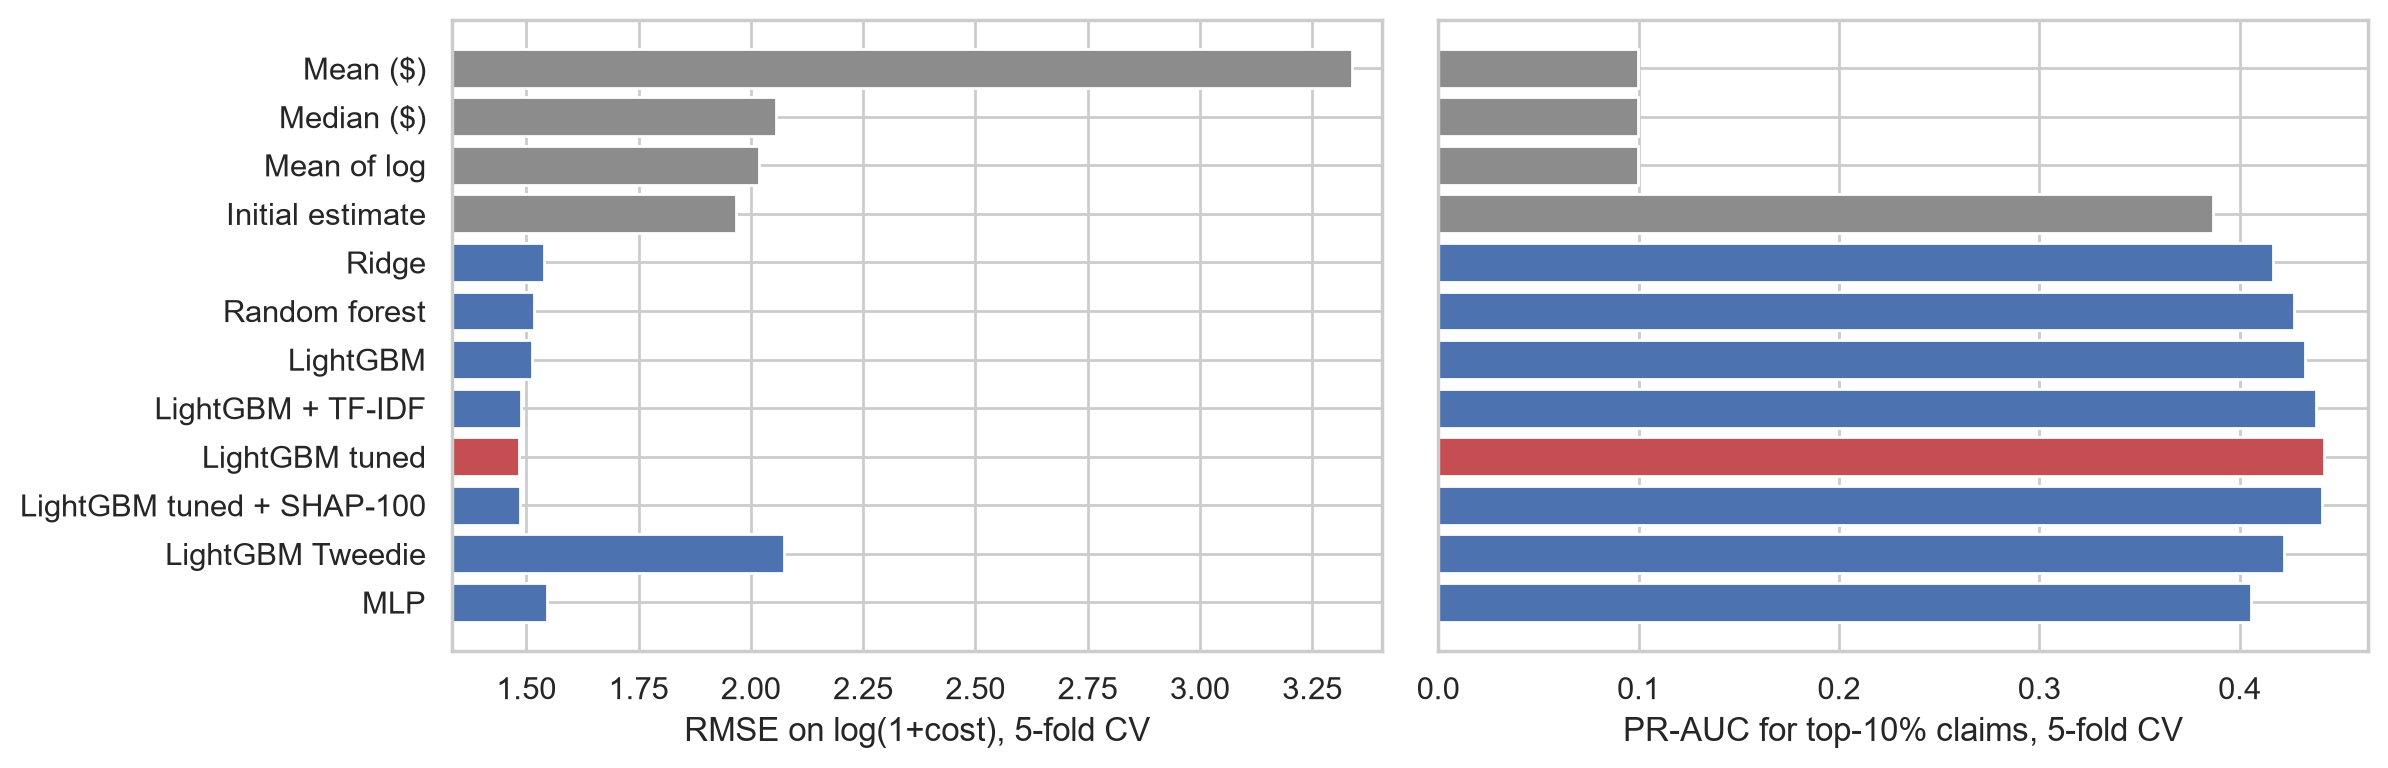
\includegraphics[width=0.85\linewidth]{fig_cv_models.png}
\caption{5-fold CV on the training set. Left: RMSE on $\log(1+\text{cost})$ (lower is better). Right: PR-AUC for the top
10\% of claims (higher is better). The champion is highlighted, baselines are grey.}
\label{fig:cv}
\end{figure*}

Table~\ref{tab:cv} and Figure~\ref{fig:cv} summarise the comparison. All learned models beat the naive baselines and the
adjuster on log-RMSE and on every triage metric. Gains come in three steps for LightGBM: tabular inputs alone (log-RMSE
1.513), adding TF-IDF text (1.488), then tuning (1.484). The tuned LightGBM is the champion under the pre-specified rule.
Its runner-up, the same model restricted to 100 SHAP-selected features, is within about 0.001 log-RMSE: the roughly
900 discarded features add almost nothing. The MLP and Ridge are the weakest learned models. The Tweedie model has the best dollar
$R^2$ (0.113) but a poor log-scale fit, because it targets the conditional mean rather than the median. The dedicated
classifier does not improve triage (PR-AUC 0.432 vs 0.442 for ranking by the regressor), so triage uses the regressor.

\subsection{Test set (used once)}

\begin{table}[t]
\centering
\caption{Held-out test set (20,000 claims). Triage at equal capacity: each method flags 2,000 claims.}
\label{tab:test}
\footnotesize
\setlength{\tabcolsep}{3pt}
\begin{tabular}{@{}lrrrr@{}}
\toprule
 & \textbf{Champion} & \textbf{SHAP-100} & \textbf{Adjuster} & \textbf{Median} \\
\midrule
MAE (\$)            & 10,498 & 10,512 & 12,772 & 11,168 \\
$R^2$ (dollar)      & 0.024  & 0.024  & 0.066  & $-0.048$ \\
$R^2_{\log}$        & 0.458  & 0.457  & 0.036  & $-0.039$ \\
ROC-AUC             & 0.864  & 0.863  & 0.848  & 0.500 \\
PR-AUC              & 0.450  & 0.446  & 0.388  & 0.101 \\
Precision@10\%      & 44.8\% & 45.1\% & 41.7\% & 9.9\% \\
Recall@10\%         & 44.4\% & 44.7\% & 41.3\% & 9.8\% \\
Capture@10\%        & 46.4\% & 47.0\% & 43.2\% & 9.8\% \\
\bottomrule
\end{tabular}
\end{table}

\begin{figure*}[t]
\centering
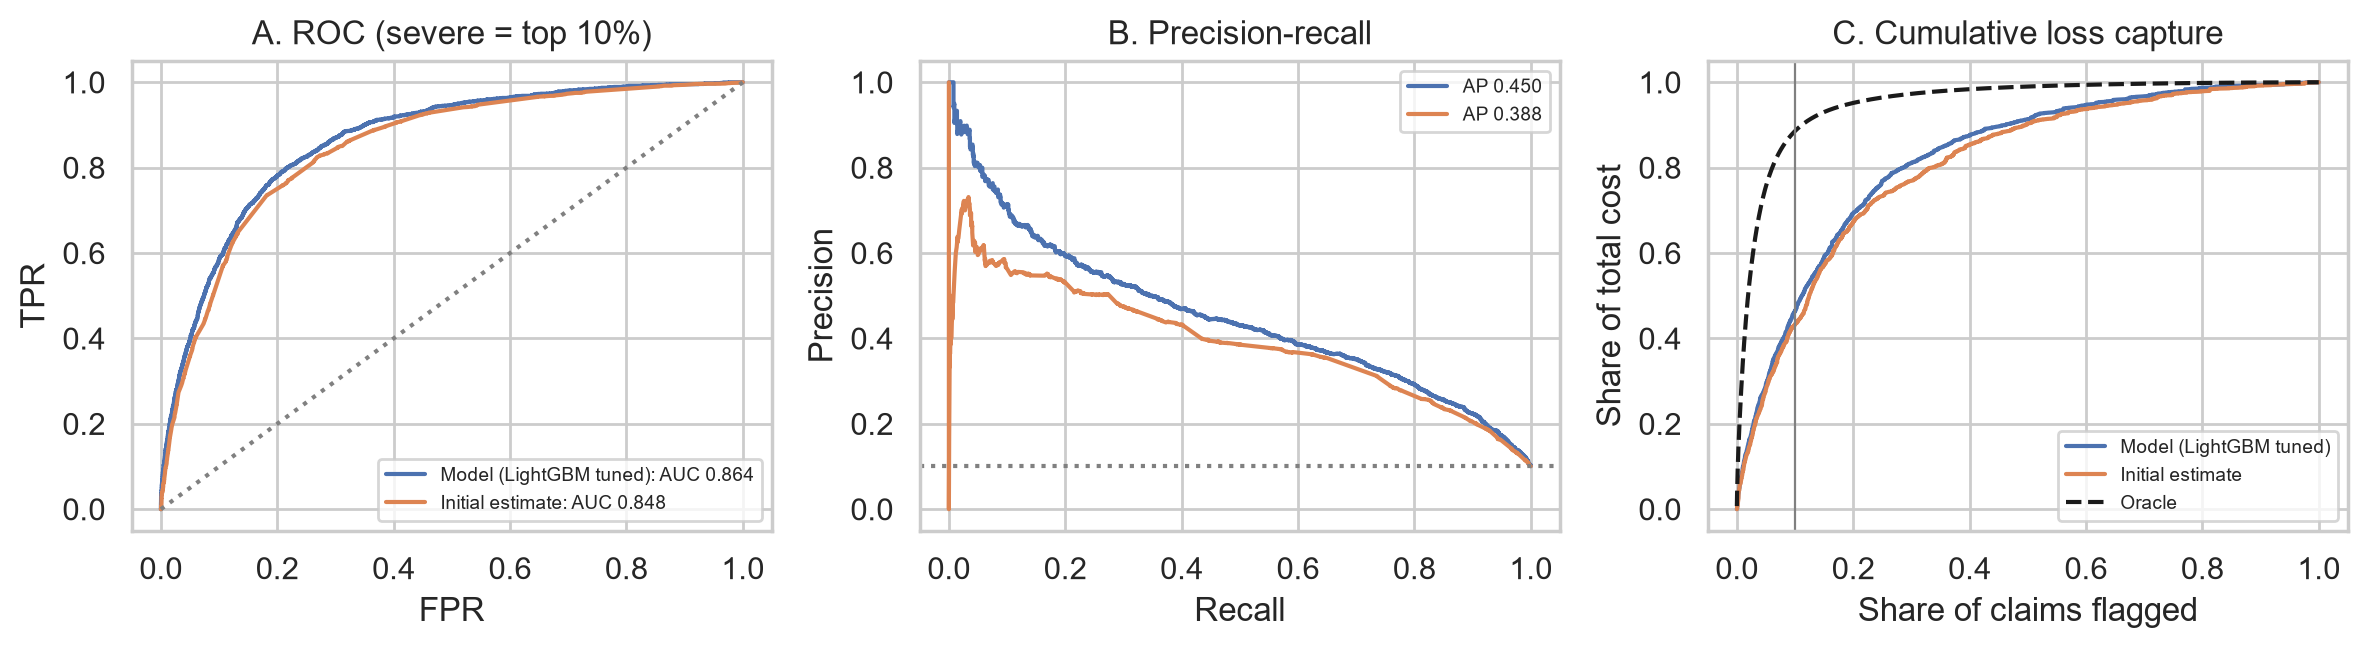
\includegraphics[width=0.92\linewidth]{fig_triage.png}
\caption{Triage on the test set: model vs adjuster's initial estimate. A: ROC curve. B: precision--recall curve. C:
cumulative share of total cost captured when claims are reviewed in decreasing order of score; the dashed line is the
oracle (ranking by true cost) and the vertical line marks the 10\% capacity.}
\label{fig:triage}
\end{figure*}

Table~\ref{tab:test} confirms the CV results. The champion explains 45.8\% of the log-cost variance and reduces the MAE
by 6.0\% relative to the median baseline. For triage (Figure~\ref{fig:triage}), at the same capacity of 2,000 reviews the
model finds 895 of the 2,016 severe claims, a lift of 4.4 over random review, against 4.1 for the adjuster. The flagged
claims carry 46.4\% of total cost against 43.2\% for the adjuster, i.e.\ about \$7.3M more of the \$227.9M test portfolio.
The champion and the SHAP-100 model cannot be distinguished on the test set: the paired bootstrap 95\% intervals of their
differences contain zero for log-RMSE ($-0.0017$ [$-0.0035$, $0.0001$]), MAE ($-\$13$ [$-\$27$, $\$0$]) and capture
($-0.5$ pts [$-1.4$, $+0.4$]).

\subsection{From log predictions to dollar totals}

\begin{figure}[t]
\centering
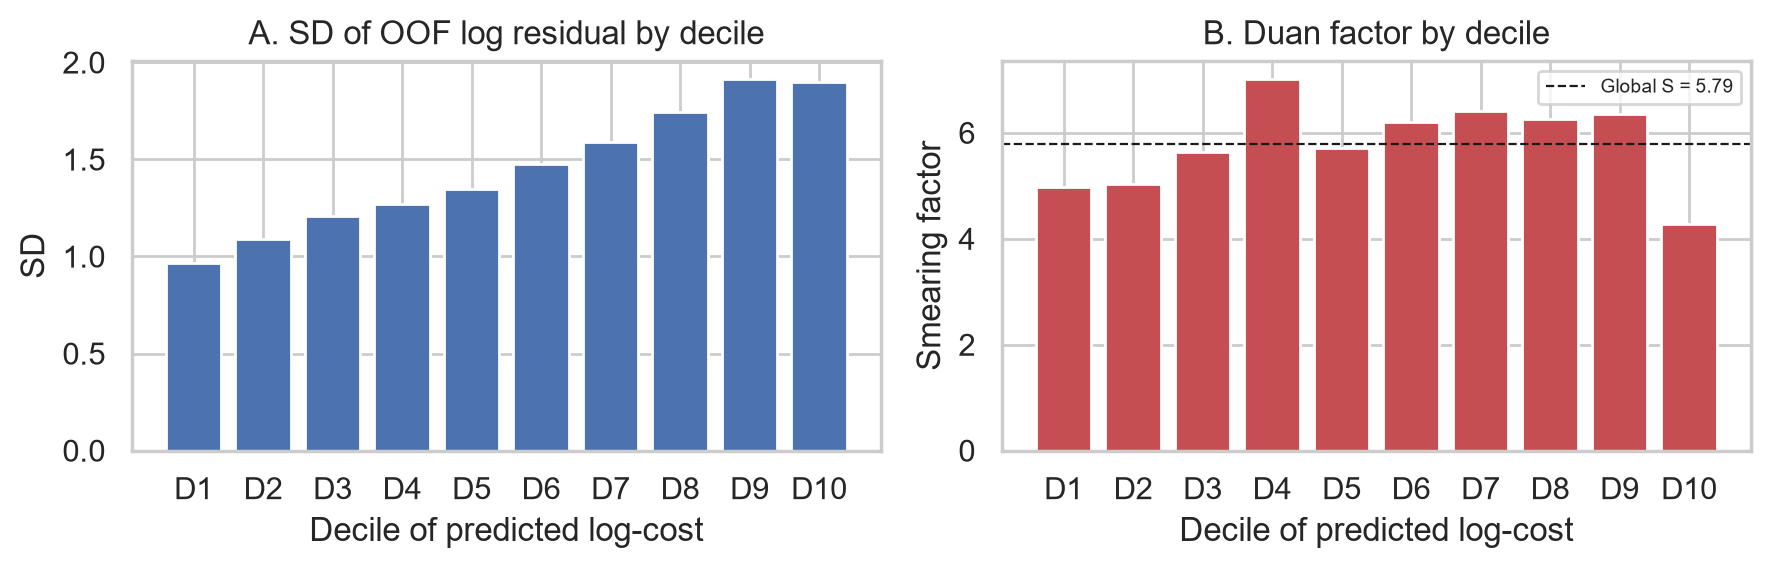
\includegraphics[width=\columnwidth]{fig_smearing.png}
\caption{Out-of-fold residuals of the champion on the training set, by decile of the predicted log-cost. A: residual
standard deviation. B: Duan smearing factor per decile; the dashed line is the global factor.}
\label{fig:smearing}
\end{figure}

\begin{table}[t]
\centering
\caption{Sum of predicted costs on the test set (actual total \$227.9M).}
\label{tab:totals}
\footnotesize
\begin{tabular}{@{}lrr@{}}
\toprule
\textbf{Method} & \textbf{Total (\$M)} & \textbf{Ratio to actual} \\
\midrule
Champion, $e^{\hat z}-1$            & 47.8  & 0.21 \\
Champion, global Duan smearing      & 276.7 & 1.21 \\
Champion, smearing per decile       & 243.5 & 1.07 \\
LightGBM Tweedie (dollar scale)     & 205.2 & 0.90 \\
Adjuster's initial estimates        & 162.4 & 0.71 \\
\bottomrule
\end{tabular}
\end{table}

Exponentiating a prediction of the log-cost gives a median-like value, not the mean. Summed over the test portfolio, it
recovers only 21\% of the actual total (Table~\ref{tab:totals}). Duan's smearing assumes that log residuals have the same
distribution whatever the prediction. That assumption fails here: the residual standard deviation doubles from 0.97 in the
lowest decile of predictions to 1.91 in the highest, and the decile-specific factors range from 4.3 to 7.0
(Figure~\ref{fig:smearing}). A single factor ($S=5.79$) therefore over-corrects (ratio 1.21) and raises the test MAE to
\$15,865. A factor per decile brings the total to 1.07, and the Tweedie model, fitted directly on dollars, to 0.90; both
also have the best dollar $R^2$ (0.096 and 0.107). For comparison, the adjusters' initial estimates cover 71\% of the
eventual total.

\subsection{Temporal drift}

\begin{table}[t]
\centering
\caption{Temporal check inside the training set: random vs chronological validation of the same size (16,000 claims).}
\label{tab:temporal}
\footnotesize
\begin{tabular}{@{}lrr@{}}
\toprule
 & \textbf{Random} & \textbf{Temporal} \\
\midrule
MAE (\$)                  & 9,971  & 20,176 \\
$R^2_{\log}$              & 0.453  & 0.400  \\
Mean log residual         & $+0.010$ & $+0.126$ \\
ROC-AUC                   & 0.857  & 0.849  \\
PR-AUC                    & 0.419  & 0.600  \\
Severe prevalence         & 9.8\%  & 23.3\% \\
PR-AUC / prevalence       & 4.26   & 2.58   \\
Capture@10\%              & 45.9\% & 37.9\% \\
\bottomrule
\end{tabular}
\end{table}

Table~\ref{tab:temporal} reports the check. Inside the training set, a model fitted on the earliest 80\% of claims by accident date and validated on the latest
20\% has twice the MAE of a random split of the same size (\$20,176 vs \$9,971), and its mean log residual moves from
$+0.010$ to $+0.126$: recent claims are systematically under-predicted. The PR-AUC looks higher in the temporal split
(0.600 vs 0.419), but the share of severe claims is also much higher there (23.3\% vs 9.8\%), because costs rise with
accident year and the threshold comes from the earlier period. Relative to prevalence, the PR-AUC falls from 4.26 to
2.58 times the random level, and loss capture from 45.9\% to 37.9\%.

\subsection{Fairness check}

\begin{table}[t]
\centering
\caption{Training-set OOF calibration (mean log residual) and flag rate by group, with and without \texttt{Gender},
\texttt{MaritalStatus} and \texttt{Age}.}
\label{tab:fair}
\footnotesize
\setlength{\tabcolsep}{2.5pt}
\begin{tabular}{@{}lrrrrr@{}}
\toprule
\textbf{Group} & \textbf{Severe} & \multicolumn{2}{c}{\textbf{Flag rate}} & \multicolumn{2}{c}{\textbf{Mean residual}} \\
 & \textbf{rate} & with & without & with & without \\
\midrule
Gender F            & 14.1\% & 13.9\% & 13.0\% & $+0.004$ & $+0.061$ \\
Gender M            & 8.8\%  & 8.8\%  & 9.1\%  & $-0.000$ & $-0.018$ \\
Marital M           & 11.4\% & 12.1\% & 10.1\% & $+0.004$ & $+0.130$ \\
Marital S           & 7.9\%  & 7.5\%  & 8.3\%  & $+0.002$ & $-0.065$ \\
Marital U           & 14.4\% & 13.6\% & 18.2\% & $-0.020$ & $-0.212$ \\
Age $<30$           & 5.9\%  & 4.1\%  & 6.2\%  & $+0.004$ & $-0.124$ \\
Age 30--44          & 11.2\% & 11.5\% & 11.0\% & $-0.005$ & $+0.043$ \\
Age 45--59          & 15.7\% & 18.4\% & 15.4\% & $+0.006$ & $+0.169$ \\
Age $\ge 60$        & 18.9\% & 23.3\% & 19.1\% & $-0.017$ & $+0.194$ \\
\bottomrule
\end{tabular}
\end{table}

With the three attributes, the model is calibrated in every group: all mean log residuals are within $\pm0.02$
(Table~\ref{tab:fair}). Without them, calibration deteriorates sharply: claims of workers aged 60 and over become
under-predicted by $+0.19$ on the log scale (about 21\% in cost), those of workers under 30 over-predicted by $-0.12$, and
claims with unknown marital status over-predicted by $-0.21$. Flag rates shift accordingly: age groups end up closer
to their true severe rates, but claims with unknown marital status become over-flagged (18.2\% flagged vs 14.4\%
severe).

\subsection{Text clusters}

\begin{table}[t]
\centering
\caption{Selected $k$-means clusters ($k=12$, training set), labelled by their top TF-IDF terms.}
\label{tab:clusters}
\footnotesize
\setlength{\tabcolsep}{3pt}
\begin{tabular}{@{}lrrrr@{}}
\toprule
\textbf{Top terms} & \textbf{$n$} & \textbf{Median} & \textbf{Severe} & \textbf{Median ICE} \\
\midrule
strain, lifting, lower back   & 10,959 & \$1,556 & 18.0\% & \$9,500 \\
injury, soft tissue           & 4,625  & \$1,106 & 13.9\% & \$2,400 \\
knee                          & 4,115  & \$856   & 13.5\% & \$3,428 \\
motor vehicle accident        & 1,333  & \$820   & 15.4\% & \$3,800 \\
right, left, struck, thumb    & 25,638 & \$539   & 10.0\% & \$1,500 \\
finger, index finger          & 7,937  & \$329   & 4.3\%  & \$1,000 \\
foreign body, eye             & 3,974  & \$214   & 1.1\%  & \$500 \\
eye, burn                     & 3,812  & \$211   & 1.8\%  & \$550 \\
\bottomrule
\end{tabular}
\end{table}

Table~\ref{tab:clusters} profiles the clusters. The silhouette of $k$-means on the LSA representation rises monotonically from 0.08 ($k=4$) to 0.16 ($k=20$): the
cluster structure is weak, so the pre-specified rule sets $k=12$. Clusters nevertheless separate injury types with very
different costs. The ``lifting / lower back strain'' cluster (10,959 claims) has the highest median cost (\$1,556) and an
18.0\% severe rate; ``motor vehicle accident'' (1,333 claims) 15.4\%; ``soft tissue injury'' 13.9\%; ``knee'' 13.5\%. At
the other end, ``foreign body in the eye'' and ``eye / burn'' have median costs of about \$210 and severe rates below 2\%.
The median ICE follows the same order, so adjusters already price injury type; the clusters mainly confirm that the text
carries information consistent with the costs.

\subsection{Failure modes}
Errors follow regression toward the median: the cheapest decile of test claims is over-predicted by $+1.60$ on the log
scale and the most expensive decile under-predicted by $-2.55$; that top decile accounts for about 88\% of the
absolute dollar error. Of the 2,016 severe test claims, 1,121 are not flagged. Their profile points to the adjuster's estimate: 10.5\% of
missed severe claims had an ICE below the training median, against none of the flagged ones. The five largest misses
(actual costs between \$0.77M and \$1.67M) all had initial estimates between \$500 and \$25,500 and ordinary descriptions,
e.g.\ ``UNLOADING GLASS STRAINED LOWER BACK'' (ICE \$25,500, prediction \$3,656, actual \$1.67M) or ``REACHED INTO GRINDER
LACERATION LEFT HIP'' (ICE \$500, actual \$0.78M).

% =====================================================================
\section{Interpretation}

\begin{figure}[t]
\centering
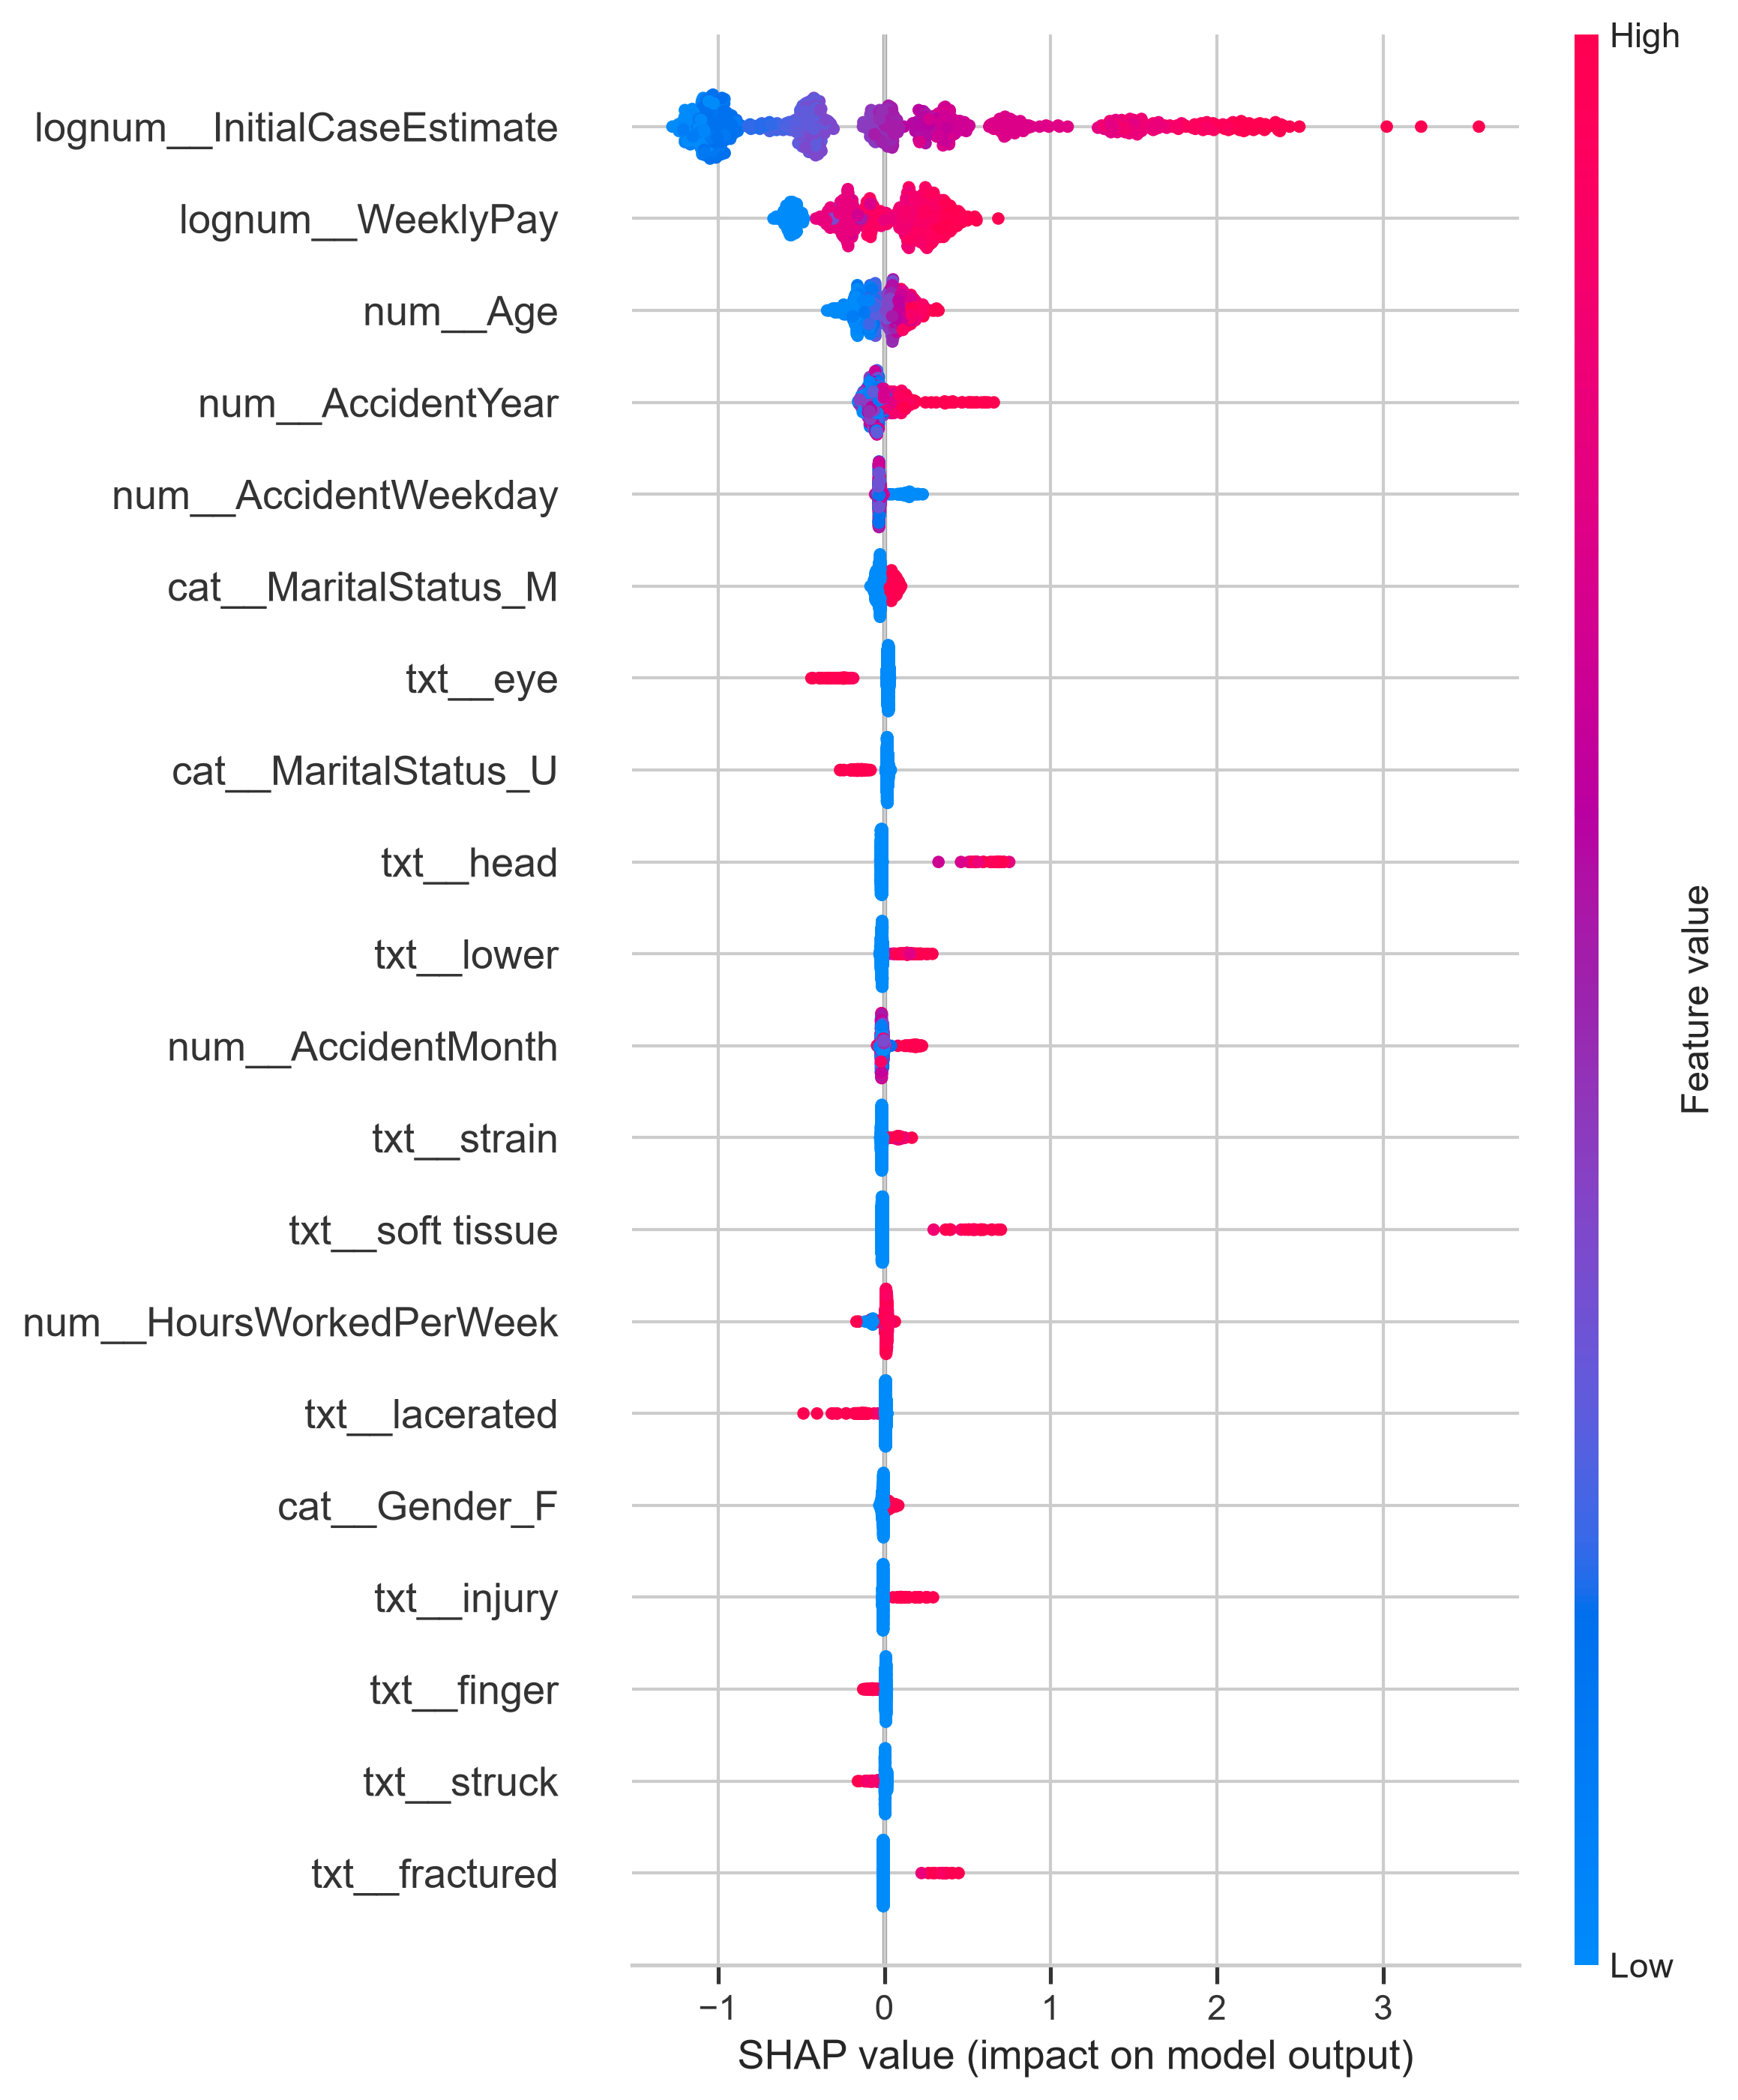
\includegraphics[width=0.92\columnwidth]{fig_shap_summary.png}
\caption{TreeSHAP summary of the champion on 1,000 training claims (log-cost scale). Each dot is a claim; colour is the
feature value.}
\label{fig:shap}
\end{figure}

\paragraph{What drives the predictions.} The SHAP summary (Figure~\ref{fig:shap}) is dominated by the adjuster's initial
estimate, whose contributions span about $-1$ to $+3.5$ on the log scale; a high ICE pushes the prediction up strongly.
Weekly pay comes second (higher pay, higher cost, consistent with wage-replacement benefits), followed by age (older
workers, higher cost) and accident year (more recent, higher cost, consistent with the drift above). Text terms act as
targeted corrections: ``head'', ``soft tissue'', ``fractured'', ``lower'' and ``strain'' increase the prediction, while
``eye'', ``lacerated'', ``finger'' and ``struck'' decrease it. These directions match the cluster profiles, which were
obtained without labels.

\begin{figure}[t]
\centering
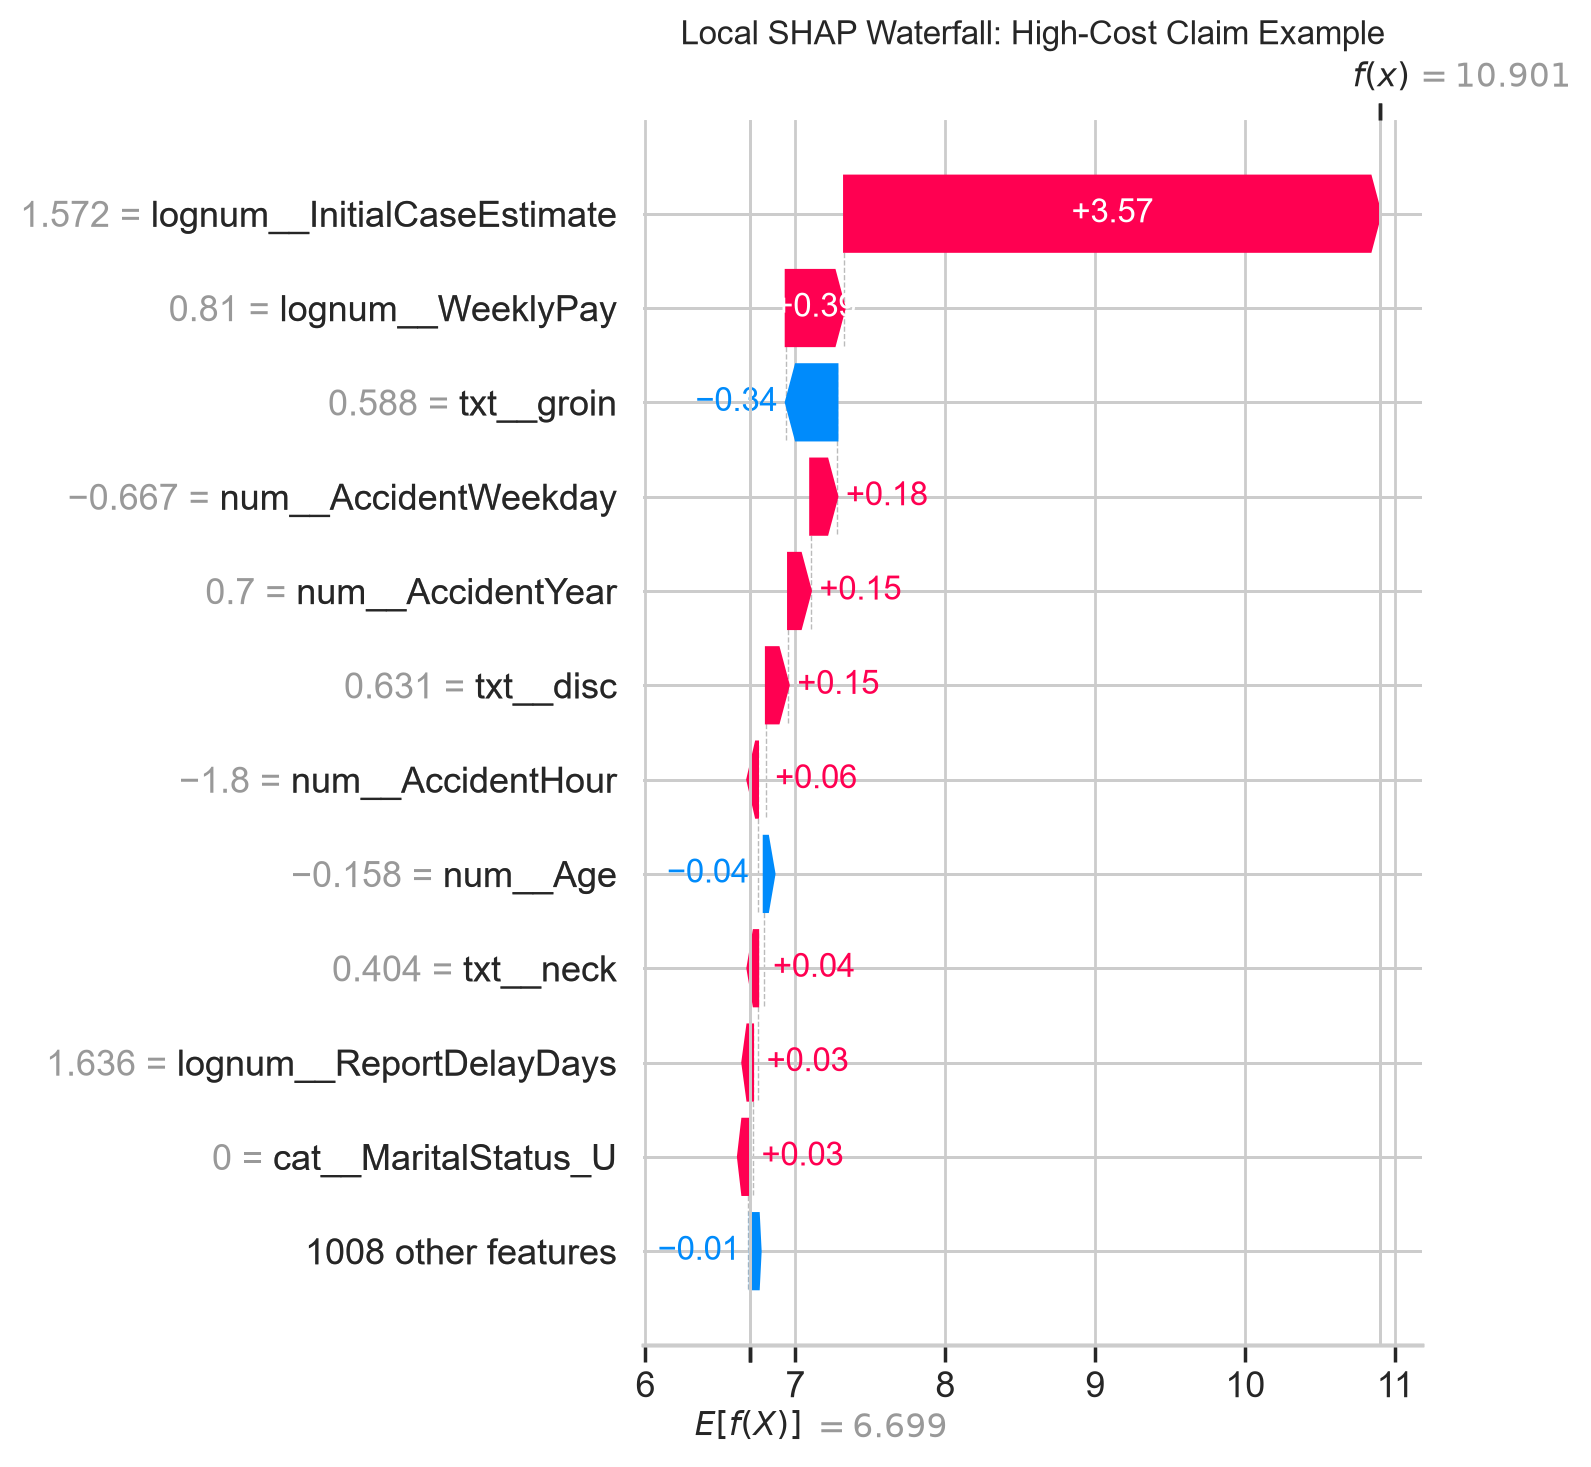
\includegraphics[width=0.92\columnwidth]{fig_shap_waterfall.png}
\caption{Local TreeSHAP explanation of the highest prediction in the SHAP sample (log-cost scale). Starting from the
average prediction $E[f(X)]=6.70$, the initial estimate adds $+3.57$; pay, accident weekday and year, and the terms
``disc'' and ``neck'' add smaller amounts, while ``groin'' lowers it.}
\label{fig:waterfall}
\end{figure}

\paragraph{Local explanations.} Figure~\ref{fig:waterfall} decomposes one high prediction. Most of it comes from a high
initial estimate (+3.57 on the log scale); the other inputs adjust it by a few tenths. This is the explanation an adjuster
would see next to a flag: it shows which facts of the file drive the score.

\paragraph{Why the model beats the adjuster, and where it does not.} The model starts from the adjuster's estimate and
corrects it with pay, age, date and injury type. This lifts the ranking of severe claims (PR-AUC $+0.06$) and recovers
claims the adjuster under-reserved but whose other attributes are typical of expensive claims. It cannot recover a claim
whose estimate, pay and description all look routine: the five largest misses are of this kind. Their eventual cost is
driven by what happens after reporting, which the data does not contain. The model is therefore a complement to the
adjuster rather than a replacement.

\paragraph{Why two models.} The selection rule picks a model of the conditional median, which is the right tool to
\emph{rank} claims; triage metrics do not depend on any smearing. Reserving needs the conditional \emph{mean}: for
portfolio totals, the Tweedie model or the decile-smeared champion should be used. The global Duan correction is not
appropriate here because the residuals are heteroscedastic.

\paragraph{Fairness.} Removing sensitive attributes breaks group calibration, because age and marital status are correlated with cost and with other inputs. Dropping them does not remove
their information; it moves the error onto the groups they describe (proxy or omitted-variable effect). ``Fairness through
unawareness'' is therefore not sufficient. Whether calibration within groups or equal flag rates should prevail is a
regulatory choice that this project does not settle.

\paragraph{Operational value.} With a hypothetical review cost $c$, reviewing the 2,000 flagged claims pays off if it
reduces their cost by $c \cdot 2{,}000$ divided by their total cost: 0.19\% for $c=\$100$, 1.9\% for $c=\$1{,}000$ and
5.7\% for $c=\$3{,}000$, slightly lower than for the adjuster's ranking (0.20\%, 2.0\%, 6.1\%). These are break-even
thresholds under illustrative costs, not estimated savings.

% =====================================================================
\section{Limitations}
\begin{itemize}
    \item \textbf{Synthetic data.} Results describe a synthetic portfolio; currency, jurisdiction and inflation are
    undocumented and costs are not deflated.
    \item \textbf{Drift.} The main protocol uses a random split; the temporal check shows that recent claims are
    under-predicted. A deployed model would need regular refitting or an explicit cost index.
    \item \textbf{Tuning.} Tuning (6 configurations) and model comparison use the same training data without nested CV,
    so the tuned model's CV score is slightly optimistic. The gap to the untuned LightGBM is small (0.004 log-RMSE).
    \item \textbf{Text models.} Text is represented by TF-IDF and LSA. Transformer embeddings (DistilBERT) were explored
    during the project, but their evaluation was not part of the leak-proof CV protocol, so we do not report them.
    \item \textbf{Uncertainty.} Test-set intervals are reported for the champion vs runner-up comparison; the
    model--adjuster comparison is supported by the consistency between CV and test rather than by a bootstrap interval.
    \item \textbf{Fixed choices.} The 90th-percentile severity threshold and the 10\% review capacity are business
    choices; other values change the figures.
\end{itemize}

% =====================================================================
\section{Conclusion}
With leak-proof cross-validation and a single use of the test set, a tuned LightGBM on tabular features and TF-IDF text
predicts the log-cost of workers' compensation claims at FNOL with $R^2_{\log}=0.46$, and ranks severe claims better
than the adjuster's initial estimate (ROC-AUC 0.864 vs 0.848; PR-AUC 0.450 vs 0.388; 46.4\% vs 43.2\% of total cost
captured at equal review capacity). Pruning to 100 SHAP-selected features gives an indistinguishable model. The model
builds on the adjuster's estimate and inherits its blind spots. For reserving, a dollar-scale Tweedie model or a smearing
per decile is required, since the naive back-transform recovers only 21\% of the total. We recommend using the model as
a decision aid for triage at intake, refitted regularly to follow cost drift, with SHAP explanations given to adjusters
for each flag.

\begin{thebibliography}{9}
\bibitem{openml} OpenML, ``workers\_compensation'' (dataset 42876), \url{https://www.openml.org/d/42876}.
\bibitem{cas2020} Casualty Actuarial Society, ``Actuarial organizations launch global data science competition,''
\url{https://www.casact.org/article/actuarial-organizations-launch-global-data-science-competition}.
\bibitem{ke2017lightgbm} G. Ke et al., ``LightGBM: A highly efficient gradient boosting decision tree,'' in \textit{NeurIPS}, 2017.
\bibitem{lundberg2017shap} S. M. Lundberg and S.-I. Lee, ``A unified approach to interpreting model predictions,'' in \textit{NeurIPS}, 2017.
\bibitem{duan1983} N. Duan, ``Smearing estimate: a nonparametric retransformation method,'' \textit{Journal of the American Statistical Association}, 78(383):605--610, 1983.
\bibitem{jorgensen} B. J{\o}rgensen, \textit{The Theory of Dispersion Models}, Chapman \& Hall, 1997.
\bibitem{botha2026} H. Botha, \textit{Data Mining \& Machine Learning, course material}, Reykjavik University, 2026.
\end{thebibliography}

\end{document}
